% !TeX spellcheck = de_CH
\chapter{Konzeption}
\begin{figure}[ht]
	\centering
	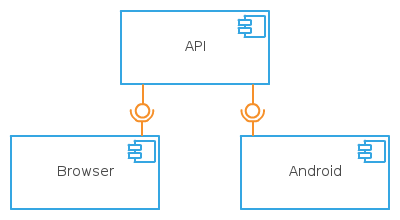
\includegraphics[width=0.7\textwidth]{Graphics/KonzeptApp.png}
	\caption{Grobkonzept f�r Applikation}
	\label{fig1}
\end{figure}
\FloatBarrier
Die Applikation besteht aus drei Teilen. Einem Webserver, der eine API und statische Clientfiles zur Verf�gung stellt, der Client im Browser, welcher die API konsumiert sowie eine Android Applikation die auch auf die API zugreift. 
 
\section{Technologiestack}
Wie in dem Grobkonzept beschrieben, wird f�r die Applikation einen Technologiestack gebraucht, welcher einfach eine skalierbare API sowie eine gute Integration der API mit einer Browser Frontend Anwendung bietet. Folgende Anforderungen werden an den Technologiestack gestellt:
\begin{itemize}
	\item Skalierbare API
	\item Einfacher und schneller Umgang mit AJAX
	\item Gute Integration zwischen API und HTML/JS Client
	\item Responsive Design, integration mit OAUTH f�r fremdauthentisierungen
	\item Persistance Layer (Datenbankunterst�tzung)
	\item Integration mit Android APIs
\end{itemize} 
\section{Applikationsdesign}
\section{DB Design}
\section{GUI Entwurf}